\documentclass[hyperref={bookmarks=false}]{beamer}
\useoutertheme{infolines}
\setbeamertemplate{headline}{} % removes the headline that infolines inserts
% \setbeamertemplate{footline}{
%   \hfill%
%   \usebeamercolor[fg]{page number in head/foot}%
%   \usebeamerfont{page number in head/foot}%
%   \insertpagenumber\,/\,\insertpresentationendpage\kern1em\vskip2pt%
% }
\setbeamertemplate{footline}{
  \hfill%
  \usebeamercolor[fg]{page number in head/foot}%
  \usebeamerfont{page number in head/foot}%
  \footnotesize\insertpagenumber\kern1em\vskip2pt%
}
\setbeamertemplate{navigation symbols}{}
\setbeamercolor{alerted text}{fg=blue}
\setbeamerfont{alerted text}{series=\bfseries,family=\ttfamily}
\setbeamertemplate{section in toc}{\text{\color{black}{\inserttocsection}}}
\usepackage[parfill]{parskip}
\usepackage{color}
\usepackage[linewidth=0.5pt]{mdframed}
\newmdenv[innerleftmargin=1mm, innerrightmargin=1mm, innertopmargin=-1mm, innerbottommargin=2mm, leftmargin=-1mm, rightmargin=-1mm]{lstlistinglike}
\usepackage{tikz}
\usepackage{graphicx}
\DeclareGraphicsExtensions{.pdf,.png,.jpg}
\usepackage{textcomp}
\usepackage{pifont}

\hypersetup{pdfauthor={Eugene Burmako},pdfsubject={Metaprogramming with Macros},pdftitle={Metaprogramming with Macros}}
\title{Scala Macros}

\begin{document}

\title{Metaprogramming with Macros}
\author{Eugene Burmako}
\institute{\'Ecole Polytechnique F\'ed\'erale de Lausanne \\
           \texttt{http://scalamacros.org/}}
\date{10 September 2012}
{
\setbeamertemplate{footline}{}
\begin{frame}
  \titlepage
\end{frame}
}

\begin{frame}[fragile]
\frametitle{What are macros?}
Macros in programming languages:
\begin{itemize}
\item C macros
\item Lisp macros
\item ...
\end{itemize}

\vskip25pt
What is the underlying notion?
\vskip25pt
\pause

The notion of textual abstraction:
\begin{itemize}
\item Recognize pieces of text that match a specification
\item Replace them according to a procedure
\end{itemize}
\end{frame}

\begin{frame}[fragile]
\frametitle{What are macros?}
\begin{semiverbatim}
printf("Hello %s!", "World")
\end{semiverbatim}

\hskip70pt
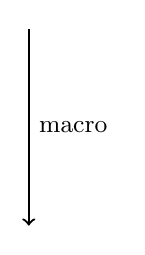
\begin{tikzpicture}
\draw[line width=0.8pt] [->] (0.0, 0.0) -- (0.0, -2.5) node[pos=0.5, right] {\small{macro}};
\end{tikzpicture}

\begin{semiverbatim}
def formatter(arg1: Any) = "Hello " + arg1.toString + "!"
print(formatter("World"))
\end{semiverbatim}
\end{frame}

\begin{frame}[fragile]
\frametitle{Why macros?}

Work with lexical tokens or syntax trees, therefore are not bound by the semantics of the underlying
programming language

Use cases:
\begin{itemize}
\item Deeply embedded DSLs (database access, testing)
\item Optimization (programmable inlining, fusion)
\item Analysis (integrated proof-checker)
\item Effects (effect containment and propagation)
\item ...
\end{itemize}
\end{frame}

\begin{frame}[fragile]
\frametitle{Challenges in macrology}

\begin{itemize}
\item Notation
\item \text{\color{blue}{Variable capture}}
\item Typechecking
\item Syntax extensibility
\item ...
\end{itemize}
\end{frame}

\begin{frame}[fragile]
\frametitle{The focus of this talk}

Inadvertent variable capture:
\begin{itemize}
\item Macro expansions sometimes cause name clashes
\item Some identifiers end up referring to variables from other scopes
\end{itemize}

\end{frame}

% \begin{frame}[fragile]
% \frametitle{Alexandre Dumas}

% \begin{center}
% \includegraphics[width=5.5cm]{dumas}
% \end{center}
% \end{frame}

\begin{frame}
\frametitle{Outline}
\tableofcontents
\end{frame}

\begin{frame}[fragile]
\frametitle{A detour: how Lisp works}
\begin{semiverbatim}
(if (calculate)
  (print "success")
  (error "does not compute"))
\end{semiverbatim}

\vskip50pt

\begin{itemize}
\item S-expressions: atoms and lists
\item \texttt{print} and \texttt{error} are one-argument functions
\item \texttt{calculate} is a zero-argument function
\item \texttt{if} is a special form
\item All values can be used in conditions
\end{itemize}
\end{frame}

\section{The prelude of macros: introduces the running example}

\begin{frame}[fragile]
\frametitle<1>{Anaphoric \texttt{if}}
\frametitle<2>{The \texttt{aif} macro}
\frametitle<3>{Low-level implementation}
\frametitle<4>{Quasiquoting: static template}
\frametitle<5>{Quasiquoting: dynamic holes}
\begin{semiverbatim}
(aif (calculate)
  (print it)
  (error "does not compute"))

\visible<2->{(defmacro aif args}
  \visible<3->{\only<3>{(list 'let* (list (list 'temp (car args))}}\only<4->{\alert{`}(let* ((temp \only<4>{...........)}\only<5->{\alert{,(car args)})}}
          \visible<3->{\only<3>{          (list 'it 'temp))}\only<4->{(it temp))}}
     \visible<3->{\only<3>{(list 'if 'temp}\only<4->{(if temp}}
       \visible<3->{\only<3>{(cadr args)}\only<4>{............}\only<5->{\alert{,(cadr args)}}}
       \visible<3->{\only<3>{(caddr args)))}\only<4>{............}\only<5->{\alert{,(caddr args)}})}

(let* ((temp (calculate))
       (it temp))
  (if temp
    (print it)
    (error "does not compute")))
\end{semiverbatim}
\end{frame}

\begin{frame}[fragile]
\frametitle{Macro by example (MBE)}
\begin{semiverbatim}
(aif (calculate)
  (print it)
  (error "does not compute"))

(defmacro+ aif
  \alert{(aif cond then else)}
  (let* ((temp \alert{cond})
         (it temp))
    (if temp
        \alert{then}
        \alert{else})))

(let* ((temp (calculate))
       (it temp))
  (if temp
    (print it)
    (error "does not compute")))
\end{semiverbatim}
\end{frame}

\begin{frame}[fragile]
\frametitle{Interlude}

\begin{semiverbatim}
(defmacro+ aif
  (aif cond then else)
  (let* ((temp cond)
         (it temp))
    (if temp then else)))
\end{semiverbatim}

\vskip50pt

\begin{itemize}
\item Macros are functions that transform syntax objects
\item Quasiquotes = static templates + dynamic holes
\end{itemize}
\end{frame}

\section{The chapter of bindings: illustrates the problem of variable capture}

\begin{frame}[fragile]
\frametitle{The \texttt{aif} macro is buggy}
\begin{semiverbatim}
\text{\color{blue}{(aif (calculate)}}
  \text{\color{blue}{(print it)}}
  \text{\color{blue}{(error "does not compute"))}}

(defmacro+ aif
  (aif cond then else)
  \text{\color{red}{(let* ((temp cond)}}
         \text{\color{red}{(it temp))}}
    \text{\color{red}{(if temp then else))}})

\visible<2>{\text{\color{red}{(let* ((temp \text{\color{blue}{(calculate)}})}}}
       \visible<2>{\text{\color{red}{(it temp))}}}
  \visible<2>{\text{\color{red}{(if temp}}}
    \visible<2>{\text{\color{blue}{(print it)}}}
    \visible<2>{\text{\color{blue}{(error "does not compute")}}\text{\color{red}{))}}}
\end{semiverbatim}
\end{frame}

\begin{frame}[fragile]
\frametitle{Bug \#1: Violation of hygiene}
\begin{semiverbatim}
(let ((\text{\color{blue}{temp}} 451{\textdegree}F))
  (aif (calculate)
    (print it)
    (print \text{\color{blue}{temp}})))

(defmacro+ aif
  (aif cond then else)
  (let* ((\text{\color{red}{temp}} cond)
         (it temp))
    (if temp then \text{\color{red}{else}})))

(let ((\text{\color{blue}{temp}} 451{\textdegree}F))
  (let* ((\text{\color{red}{temp}} (calculate))
         (it temp))
    (if temp
      (print it)
      (print \text{\color{red}{temp}}))))
\end{semiverbatim}
\end{frame}

\begin{frame}[fragile]
\frametitle{Bug \#2: Violation of referential transparency}
\begin{semiverbatim}
(let ((\text{\color{blue}{if hijacked}}))
  (aif (calculate)
    (print it)
    (error "does not compute")))

(defmacro+ aif
  (aif cond then else)
  (let* ((temp cond)
         (it temp))
    (\text{\color{red}{if}} temp then else))) \text{\color{red}{;; core if}}

(let ((\text{\color{blue}{if hijacked}}))
  (let* ((temp (calculate))
         (it temp))
    (\text{\color{blue}{if}} temp \text{\color{blue}{;; hijacked if}}
      (print it)
      (error "does not compute"))))
\end{semiverbatim}
\end{frame}

\begin{frame}[fragile]
\frametitle{Old school solution}
\begin{semiverbatim}
(defmacro+ aif
  (aif cond then else)
  \alert{(let ((temp (gensym)))}
    (let* ((temp cond)
           (it temp))
      (if temp then else))))
\end{semiverbatim}

\text{\color{blue}{Packages help with referential transparency}}
\end{frame}

\section{The trilogy of tongues: surveys macro systems that solve this problem}

\begin{frame}[fragile]
\frametitle{Three macro-enabled languages}

\emph{Template Meta-programming for Haskell} \text{\color{blue}{[Template Haskell]}}\\
by Tim Sheard and Simon Peyton Jones

\vskip15pt

\emph{Meta-programming in Nemerle} \text{\color{blue}{[Nemerle]}}\\
by Kamil Skalski, Michal Moskal and Pawel Olszta.

\vskip15pt

\emph{Keeping it Clean with Syntax Parameters} \text{\color{blue}{[Racket]}}\\
by Eli Barzilay, Ryan Culpepper and Matthew Flatt

\vskip15pt

All three languages:
\begin{itemize}
\item Solve the problems of hygiene and referential transparency
\item Do that in their own interesting ways
\end{itemize}
\end{frame}

\begin{frame}[fragile]
\frametitle<1>{Template Haskell: Introduction}
\frametitle<2>{Template Haskell: The perils of hygiene}
\begin{semiverbatim}
{\textdollar}(aif [| calculate |]
  [| putStrLn (show \text{\color<2->{blue}{it}}) |]
  [| error "does not compute" |])

aif :: Q Exp -> Q Exp -> Q Exp -> Q Exp
aif cond then' else' =
  [| let temp = {\textdollar}cond
         \text{\color<2->{red}{it}} = temp
     in if temp /= 0 then {\textdollar}then' else {\textdollar}else' |]
\only<2->{
let temp_a1mx = calculate
    \text{\color{red}{it_a1my}} = temp_a1mx
in if (temp_a1mx /= 0)
   then putStrLn (show \text{\color{blue}{it}})
   else error "does not compute"

\text{\color{blue}{Not in scope: `it'}}}
\end{semiverbatim}

\only<1>{
\begin{itemize}
\item No dedicated concept of macros
\item Macro expansions are triggered explicitly with \texttt{\textdollar}
\item There are quasiquotes \texttt{[| ...\ |]} and unquotes \texttt{{\textdollar}expr}
\item Hygienic and referentially transparent
\end{itemize}
\vskip14pt
}
\end{frame}

\begin{frame}[fragile]
\frametitle{Template Haskell: The \texttt{Q} monad}
\begin{semiverbatim}
aif cond then' else' =
  [| let \text{\color{blue}{temp = {\textdollar}cond}}
         \text{\color{blue}{it = temp}}
     in if temp \text{\color{red}{/=}} 0 then {\textdollar}then' else {\textdollar}else' |]

aif :: Q Exp -> Q Exp -> Q Exp -> Q Exp
aif cond' then'' else'' =
    do \{ ...
       ; \text{\color{blue}{temp <- newName "temp"}}
       ; \text{\color{blue}{it <- newName "it"}}
       ; \text{\color{red}{let notEq = mkNameG_v "ghc-prim" "GHC.Classes" "/="}}
         in return (LetE ... (CondE (... then' else')) ...)
       \}
\end{semiverbatim}
          % (LetE [ValD (VarP temp) (NormalB cond) [],
          %        ValD (VarP it) (NormalB (VarE temp)) []]
          %       (CondE (... (VarE notEq) ...) then' else'))
          %       (CondE (InfixE (Just (VarE temp)) (VarE notEq) (Just (LitE (IntegerL 0)))) then' else'))
\end{frame}

\begin{frame}[fragile]
\frametitle{Template Haskell: Breaking hygiene}
\begin{semiverbatim}
{\textdollar}(aif [| calculate |]
  [| putStrLn (show \alert{{\textdollar}(dyn "it")}) |]
  [| error "does not compute" |])

aif :: Q Exp -> Q Exp -> Q Exp -> Q Exp
aif cond then' else' =
  [| let temp = {\textdollar}cond
         \text{\color{red}{it}} = temp
     in if temp /= 0 then {\textdollar}then' else {\textdollar}else' |]

let temp_a1mx = calculate
    \text{\color{red}{it_a1my}} = temp_a1mx
in if (temp_a1mx /= 0)
   then putStrLn (show \text{\color{blue}{it_a1my}})
   else error "does not compute"
\end{semiverbatim}
\end{frame}

\begin{frame}[fragile]
\frametitle{Template Haskell: Summary}
\begin{itemize}
\item Template Haskell is auto hygienic and referentially transparent
\item The Q monad takes care of names
\item \text{\color{blue}{Sometimes we need to break hygiene}}
\end{itemize}
\end{frame}

\begin{frame}[fragile]
\frametitle<1>{Nemerle: Introduction}
\frametitle<2>{Nemerle: The perils of hygiene}
\begin{semiverbatim}
aif(calculate,
  WriteLine(\text{\color<2->{blue}{it}}),
  throw Exception("does not compute"))

macro aif(cond, then, else_) \{
  <[
    def temp = {\textdollar}cond;
    def \text{\color<2->{red}{it}} = temp;
    if (temp != 0) {\textdollar}then else {\textdollar}else_
  ]>
\}
\only<2>{
def calculate = 42;
def temp_1087 = calculate;
def \text{\color{red}{it_1088}} = temp_1087;
if (temp_1087 != 0) WriteLine(\text{\color{blue}{it}}) else throw Exception("...")

\text{\color{blue}{error: unbound name `it'}}}
\end{semiverbatim}

\only<1>{
\begin{itemize}
\item Macros are declared explicitly, expansions are implicit
\item There are quasiquotes \texttt{<[ ...\ ]>} and unquotes \texttt{{\textdollar}expr}
\item Hygienic and referentially transparent
\end{itemize}
\vskip14pt
}
\end{frame}

\begin{frame}[fragile]
\frametitle<1>{Nemerle: Coloring algorithm}
\frametitle<2>{Nemerle: Coloring algorithm}%: normal code gets a vanilla color}
\frametitle<3>{Nemerle: Coloring algorithm}%: each expansion gets unique colors}
\frametitle<4>{Nemerle: Coloring algorithm}%: at the end of the day}
\frametitle<5>{Nemerle: Breaking hygiene}%: inherit use site}
\begin{semiverbatim}
def \text{\color<2-4>{blue}{calculate}} = 42;                 \only<2->{\text{\color{blue}{// vanilla color}}}
aif(\text{\color<2-4>{blue}{calculate}},
  WriteLine(\text{\color<2-5>{blue}{it}}),
  throw Exception("does not compute"))

macro aif(cond, then, else_) \{      \only<3->{\text{\color{red}{// expansion color}}}
  <[
    def \text{\color<3-4>{red}{temp}} = \text{\color<3-4>{blue}{{\textdollar}cond}};
    def \only<1,2>{it}\only<3,4>{\text{\color{red}{it}}}\only<5>{\text{\color{blue}{{\textdollar}("it": usesite)}}} = \text{\color<3-4>{red}{temp}};    \only<5->{\text{\color{blue}{// recolor the variable}}}
    if (\text{\color<3-4>{red}{temp}} != 0) \text{\color<3-4>{blue}{{\textdollar}then}} else \text{\color<3-4>{blue}{{\textdollar}else_}}
  ]>
\}

def \text{\color<4-4>{blue}{calculate}} = 42;                 \only<4->{// bind using colors}
def \text{\color<4-4>{red}{temp}} = \text{\color<4-4>{blue}{calculate}};
def \text{\color<4>{red}{\color<5>{blue}{it}}} = \text{\color<4-4>{red}{temp}};
if (\text{\color<4-4>{red}{temp}} != 0) WriteLine(\text{\color<4->{blue}{it}}) else throw Exception("...")
\end{semiverbatim}
\end{frame}

\begin{frame}[fragile]
\frametitle{Nemerle: Summary}
\begin{itemize}
\item Nemerle takes care of hygiene with a coloring algorithm
\item No complex translation algorithms are necessary
\item As another bonus programmer can fine-tune colors with \texttt{MacroColors}
\item Referential transparency works as well
\end{itemize}
\end{frame}

\begin{frame}[fragile]
\frametitle<1>{Racket: Introduction}
\frametitle<2>{Racket: The perils of hygiene}
\frametitle<3>{Racket: Breaking hygiene}
\begin{semiverbatim}
\text{\color<2->{blue}{(aif (calculate)}}
  \text{\color<2->{blue}{(print it)}}
  \text{\color<2->{blue}{(error "does not compute"))}}

(define-syntax (aif stx)
  (syntax-case stx ()
    ((aif cond then else)
     \visible<3->{(with-syntax ((\text{\color<3->{blue}{it}} (datum->syntax \text{\color<3->{blue}{#'aif}} \text{\color<3->{red}{'it}})))}
       #'(let ((temp cond)
               (\text{\color<3->{blue}{\color<2>{red}{it}}} temp)))
           (if temp then else)))))\visible<3->{)}
\only<2->{
(let* ((temp (calculate))
       (\text{\color<3->{blue}{\color<2>{red}{it}}} temp))
  (if temp
    \text{\color<2->{blue}{(print it)}}
    \text{\color<2->{blue}{(error "does not compute")}}))}
\end{semiverbatim}

\only<1>{
\begin{itemize}
\item A Lisp, descendent from Scheme
\item 25 years of hygienic macros, a bunch of macro systems
\item Language features written using macros (classes, modules, etc)
\end{itemize}
\vskip7pt
}
\end{frame}

\begin{frame}[fragile]
\frametitle<1->{Racket: The \texttt{aunless} macro}
\frametitle<2->{Racket: Being unhygienic doesn't scale}
\begin{semiverbatim}
\text{\color<3->{teal}{(aunless (not (calculate))}}
  \text{\color<3->{teal}{(print it)}}
  \text{\color<3->{teal}{(error "does not compute"))}}

(define-syntax (aunless stx)
  (syntax-case stx ()
    (\alert<1>{(aunless cond then else)}
     \text{\color<2->{blue}{\alert<1>{#'(aif (not cond) then else)}}})))

\text{\color<2->{red}{(let* ((temp (not (not (calculate))))}}
       \text{\color<2->{red}{(}}\text{\color<2->{blue}{it}} \text{\color<2->{red}{temp))}}
  \text{\color<2->{red}{(if temp}}
    \text{\color<3->{teal}{(print it)}}
    \text{\color<3->{teal}{(error "does not compute")}}))
\end{semiverbatim}
\end{frame}

\begin{frame}[fragile]
\frametitle{Racket: Syntax parameters}
\begin{semiverbatim}

\text{\color{teal}{(define-syntax-parameter it (syntax-rules ()))}}

(define-syntax (aif stx)
  (syntax-case stx ()
    ((aif cond then else)
     #'(let ((temp cond))
             \text{\color{teal}{(syntax-parameterize}}
               \text{\color{teal}{((it (syntax-rules () ((_) temp))))}}
         (if temp then else))))))

\end{semiverbatim}

\begin{itemize}
\item \texttt{it} becomes a compile-time dynamic variable
\item Therefore its scope overarches all potential expansions
\item \text{\color{blue}{High-level language feature (dynamic variables) + macros = win}}
\end{itemize}
\end{frame}

\begin{frame}[fragile]
\frametitle{Summary}
Macros:
\begin{itemize}
\item Macros provide impressive power for their simplicity
\item But they also give rise to unusual problems
\item One of these problems involves mixed up bindings
\end{itemize}

\pause
Bindings:
\begin{itemize}
\item Automatic hygiene and referential transparency are real
\item Sometimes it is necessary to break hygiene
\item There are ways of doing that
\item Sometimes these ways are too low-level
\end{itemize}

\pause
Future work:
\begin{itemize}
\item Integration with other language features provides unexpected insights
\end{itemize}
\end{frame}

\section{The vision of the days to come: presents the research proposal}

\begin{frame}[fragile]
\frametitle{Scala macros}
\begin{itemize}
\item Since this spring Scala has macros
\item Even better: macros are an official part of the language in the next production release 2.10.0
\item Now it's time to put the pens down and think about the future
\item The future is in integration with other language features
\end{itemize}
\end{frame}

\begin{frame}[fragile]
\frametitle{Implicits}
\begin{semiverbatim}
\visible<2->{trait Serializer[T] \{
  def write(pickle: Pickle, x: T): Unit
\}
}
def serialize[T](x: T)\only<2->{(\only<3->{\alert<3>{implicit }}s: Serializer[T])}: Pickle

\visible<3->{\only<1-3>{\alert<3>{implicit object ByteSerializer extends Serializer[Byte] \{
  def write(pickle: Pickle, x: Byte) = pickle.writeByte(x)
\}}}\only<4->{\visible<4->{\alert<4>{implicit def generator: Serializer[T] = macro impl[T]
def impl[T](c: Context): c.Expr[Serializer[T]] = ...
}}}}
\end{semiverbatim}
\end{frame}

\begin{frame}[fragile]
\frametitle{Research proposal}

Marry macros and high-level language features:

\begin{itemize}
\item Macros + functions $\rightarrow$ programmable inlining, specialization, fusion
\item Macros + annotations $\rightarrow$ code contracts, statically-typed decorators
\item Macros + implicits $\rightarrow$ static verification
\item ...
\end{itemize}
\end{frame}

\begin{frame}[fragile]
\vskip50pt
\begin{center}
\large Backup slides
\end{center}
\end{frame}

\begin{frame}[fragile]
\frametitle{Macros for database access: SLICK}
\begin{semiverbatim}
@table("COFFEES") case class Coffee(
  @column("COF_NAME") name: String,
  @column("SUP_ID") supID: Int,
  @column("PRICE") price: Double
)
val coffees = Queryable[Coffee]

val l = for \{ c <- coffees if c.supID == 101 \}
yield (c.name, c.price)

backend.result(l, session)
 .foreach \{ case (n, p) => println(n + ": " + p) \}
\end{semiverbatim}

\begin{itemize}
\item Deeply embedded domain-specific language
\item Constructs like field access and method calls are overloaded
\item Underlying macros save ASTs till runtime and translate them to SQL
\end{itemize}
\end{frame}

\begin{frame}[fragile]
\frametitle{Macros for testing: ScalaMock}
\begin{semiverbatim}
val w = mock[Warehouse]
inSequence \{
  w.expects.hasInventory("Talisker", 50).returning(true)
  w.expects.remove("Talisker", 50).once
\}

val order = new Order("Talisker", 50)
order.fill(w)
assert(order.isFilled)

\end{semiverbatim}

\begin{itemize}
\item Deeply-embedded domain-specific language
\item Macro types generate mocks at compile-time
\item Boilerplate generation is completely automatic
\end{itemize}
\end{frame}

\begin{frame}[fragile]
\frametitle{Macros for inlining: Scala collections}
\begin{semiverbatim}
def filter(p: T => Boolean): Repr = ...

def filter(p: T => Boolean): Repr = macro inline \{
  ... the original body of filter ...
\}

\end{semiverbatim}

\begin{itemize}
\item The \texttt{filter} function transparently becomes a macro
\item This doesn't break source compatibility
\item The original body of \texttt{filter} remains the same
\item Yet the underlying macro is now in full control of inlining
\end{itemize}
\end{frame}

\begin{frame}[fragile]
\frametitle{Macros for fusion: Courtesy of Paul Phillips}
\begin{semiverbatim}
def inc(x: Int) = x + 1
def f = List(1, 2, 3) map inc map inc map inc
def g = List(1, 2, 3) map inc map inc map inc fuse

\end{semiverbatim}

\begin{itemize}
\item Desktop fusion achieved!
\item How to deal with side effects?
\item Also what about data flow analysis?
\end{itemize}
\end{frame}

\begin{frame}[fragile]
\frametitle{Macros for verification: Courtesy of Alexander Kuklev}
\begin{semiverbatim}
trait SemiGroup[T] extends Eq[T] \{
  def \ensuremath{\circ}(a: T, b: T): T
  def associativity(a: T, b: T, c: T):
    \ding{51}((a \ensuremath{\circ} (b \ensuremath{\circ} c)) == ((a \ensuremath{\circ} b) \ensuremath{\circ} c))
\}

def reduce[T](op: (T, T) => T): T

def reduce[T](op: (T, T) => T)(implicit evidence:
  \ding{51}((a: T, b: T, c: T) => op(op(a, b), c) == op(a, op(b, c)))
): T
\end{semiverbatim}

\begin{itemize}
\item Facts are encoded with the \ding{51} macro
\item Proofs are requested with implicit parameters
\item Proofs can either be inferred by implicit macros or provided by hand
\end{itemize}
\end{frame}

\begin{frame}[fragile]
\frametitle{Scala in the present: Macro defs}
\begin{semiverbatim}
object Asserts \{
  def assertionsEnabled = ...
  def raise(msg: Any) = throw new AssertionError(msg)

  def assert(cond: Boolean, msg: Any) = macro impl
  def impl(c: Context)
          (cond: c.Expr[Boolean], msg: c.Expr[Any]) =
    if (assertionsEnabled)
      c.reify(if (!cond.eval) raise(msg.eval))
    else
      c.reify(())
\}
\end{semiverbatim}

\begin{itemize}
\item Separate macro definitions and implementations
\item \texttt{reify} ensures hygiene and referential transparency
\item \texttt{reify} also implements the notion of quasiquoting
\end{itemize}
\end{frame}

\begin{frame}[fragile]
\frametitle{Scala in the future: Type macros}
\begin{semiverbatim}
type MySqlDb(connString: String) = macro ...

type MyDb = Base with MySqlDb("Server=127.0.0.1")

import MyDb._
val products = new MyDb().products
products.filter(p => p.name.startsWith("foo")).toList

\end{semiverbatim}

\begin{itemize}
\item Generalize macros from term refs to symbol refs
\item Type macros can generate arbitrary amounts of publicly visible defs
\item Enables an astounding multitude of techniques
\item The problem of erasure
\end{itemize}
\end{frame}

\begin{frame}[fragile]
\frametitle{Scala in the future: Macro annotations}
\begin{semiverbatim}
class atomic extends MacroAnnotation \{
  def complete(defn: _) = macro("generate a backing field")
  def typeCheck(defn: _) = macro("return defn itself")
\}

@atomic var fld: Int

\end{semiverbatim}

\begin{itemize}
\item Statically-typed analogue of Python's decorators
\item Operates on arbitrary definitions
\item Two-step expansion: macro-level + micro-level
\end{itemize}
\end{frame}

\begin{frame}[fragile]
\frametitle{Typechecking disciplines: Strict}
\begin{semiverbatim}
-| fun pow n = <fn x =>
    ~(if n = 0 then <1> else <x * (~(pow (n - 1)) x)>)>;
val pow = fn : int -> <int -> int>

-| val cube = (pow 3);
val cube = <(fn a => x %* x %* x %* 1)> : <int -> int>

-| (run cube) 5;
val it = 125 : int

\end{semiverbatim}

\begin{itemize}
\item Each quasiquote is typechecked in isolation
\item All quasiquotes are assigned "code of something" types
\item E.g. right-hand side of \texttt{pow} is a code of function from \texttt{int} to \texttt{int}
\item Hence no pattern matching and no new bindings
\end{itemize}
\end{frame}

\begin{frame}[fragile]
\frametitle{Typechecking disciplines: Lenient}
\begin{semiverbatim}
[| 'a' + True |] -- rejected

printf :: String -> Expr -- allowed
{\textdollar}(printf "Error: %s on line %d") "urk" 341

f :: Q Type -> Q [Dec] -- rejected
f t = [d| data T = MkT {\textdollar}t; g (MkT x) = x + 1 |]

\end{semiverbatim}

\begin{itemize}
\item Quasiquotes are sanity-checked early, fully typechecked later
\item But require their bindings to be established in advance
\item Not flexible enough, e.g. no splicing into binding positions
\end{itemize}
\end{frame}

\begin{frame}[fragile]
\frametitle{Typechecking disciplines: Deferred}
\begin{semiverbatim}
macro using(name, expr, body) \{
  <[
    def {\textdollar}name = {\textdollar}expr;
    try \{ {\textdollar}body \} finally \{ {\textdollar}name.Dispose() \}
  ]>
\}
using(db, Database("localhost"), db.LoadData())

\end{semiverbatim}

\begin{itemize}
\item Quasiquotes are not typechecked at all
\item Typechecking only happens after macro expansion
\item This gives ultimate flexibility at the cost of delayed error detection
\end{itemize}
\end{frame}

\end{document}